\documentclass[10pt,twocolumn,letterpaper]{article}

\usepackage{cvpr}
\usepackage{xfrac}
\usepackage{times}
\usepackage{epsfig}
\usepackage{graphicx}
\usepackage{amsmath}
\usepackage{amssymb}
\usepackage{color, soul}
\usepackage{float}
\usepackage[super]{nth}
\setlength{\intextsep}{5pt}
\usepackage[nodisplayskipstretch]{setspace}
\setstretch{1}

% Include other packages here, before hyperref.

% If you comment hyperref and then uncomment it, you should delete
% egpaper.aux before re-running latex.  (Or just hit 'q' on the first latex
% run, let it finish, and you should be clear).
\usepackage[breaklinks=true,bookmarks=false]{hyperref}

\cvprfinalcopy % *** Uncomment this line for the final submission

\def\cvprPaperID{****} % *** Enter the CVPR Paper ID here
\def\httilde{\mbox{\tt\raisebox{-.5ex}{\symbol{126}}}}

% Pages are numbered in submission mode, and unnumbered in camera-ready
%\ifcvprfinal\pagestyle{empty}\fi
\setcounter{page}{1}
\begin{document}

%%%%%%%%% TITLE
\title{Pattern Recognition Coursework 1}

\author{Jakub Mateusz Szypicyn\\
CID: 00846006\\
EEE4\\
{\tt\small jms13@ic.ac.uk}
% For a paper whose authors are all at the same institution,
% omit the following lines up until the closing ``}''.
% Additional authors and addresses can be added with ``\and'',
% just like the second author.
% To save space, use either the email address or home page, not both
\and
Jacobus Jukka Hertzog\\
CID: 00828711\\
EEE4\\
{\tt\small jjh13@ic.ac.uk}
}

\maketitle
%\thispagestyle{empty}

%%%%%%%%% ABSTRACT
\begin{abstract}

Line1\\

Line3\\

Line5\\

Line7\\

\end{abstract}

%%%%%%%%% BODY TEXT
\section{Introduction}

It is often desirable to be able to quickly and accurately transform handwritten text into computer text or to assign name to a person based on their face using computer programs. The process requires the computer to have some prior knowledge of what it is trying to compute. This is known as training data. Based on the training data we can build mathematical models which will allows us to recognise faces or letters.

In this paper we are investigating and describing basic methods of training and testing, such as Principal Coefficient Analysis (PCA), Nearest Neighbour classification (NN) and multiclass Support Vector Machine (SVM) classification including binary class SVM. 

%-------------------------------------------------------------------------
\section{Eigenfaces}

\subsection{Data partition}

A Matlab file containing face data {\tt\small face.mat} has been provided for the purpose of this coursework. The file contains a $2576 \times 520$ matrix of face images. Each image is stored in a column. Given that the matrix has 520 columns there are 520 pictures of faces. Those pictures belong to 52 distinct persons. Therefore there are 10 pictures per person. Furthermore each picture has dimensions of $56 \times 46$ pixels.

In order to divide the data set into training and testing subsets, we have decide to preserve as much variance int he training data as possible. This would ensure that each set of faces is separated as far as possible, which potentially ensures higher identification rate.

The data was divided in the following ratio of testing to training: $20\%$ to $80\%$. From each set of 10 pictures we have thus taken two most average pictures, based on the average pixel values. The two sets will be heron referred to as {\tt\small training} ($2576 \times 416$ matrix) and {\tt\small testing} ($2576 \times 104$ matrix).

\subsection{PCA of face data}
\subsubsection{\boldmath$AA^T$} \label{sec:aat}
Following the algorithm for Principal Component Analysis, we have first detrended the face images by subtracting a mean vector from all columns of {\tt\small training}, which resulted in a matrix $A$, whose rows are now zero-mean. Following the above, the covariance matrix $S=\frac{1}{416} \times AA^T$ has been calculated. $S$ has dimensions of $2576 \times 2576$.

The covariance matrix $S$ uniquely describes the data by calculating its spread or variance denoted $\sigma$ and its orientation. For face recognition we would like to make use of both of those properties. Namely, we would like to identify and keep vectors along which the data spread is the largest, disposing of dimensions which do not carry any spread information. This helps us to reduce problem size, decrease memory usage and increase performance. 

The dimensions corresponding to largest data spread are given to us by calculating the eigenvalues and eigenvectors of $S$. We expect that there will be at most $416$ non-zero eigenvalues. This follows from \cite{Data Mining}. Given a rectangular matrix $A$, $S_1 = AA^T$ and $S_2 = A^TA$ share all non-zero eigenvalues. This means that the larger of the two matrices will have as many non-zero eigenvalues as the smaller one. Given that the dimensions of the smaller matrix are in our case $416 \times 416$, we expect that the larger matrix of $2576 \times 2576$ will return at most 416 non-zero eigenvalues. It of course can be the case, that there will be fewer non-zero eigenvalues. This proves to be the case with {\tt\small training}. The resulting covariance matrix produces 415 significant eigenvalues. This can be accredited to one of two things:

\begin{enumerate}
\item The data is such that variance in one of the dimensions is actually zero.
\item The precision of {\tt\small double float} calculations is insufficient. Since the data is very large, none of the 'zero' eigenvalues are actually equal to zero. They are however very small varying between $10^{-10}$ and $10^{-14}$. This is shown in Figure \ref{fig:Eig1} below.
\end{enumerate}

\begin{figure}[H]

\centering
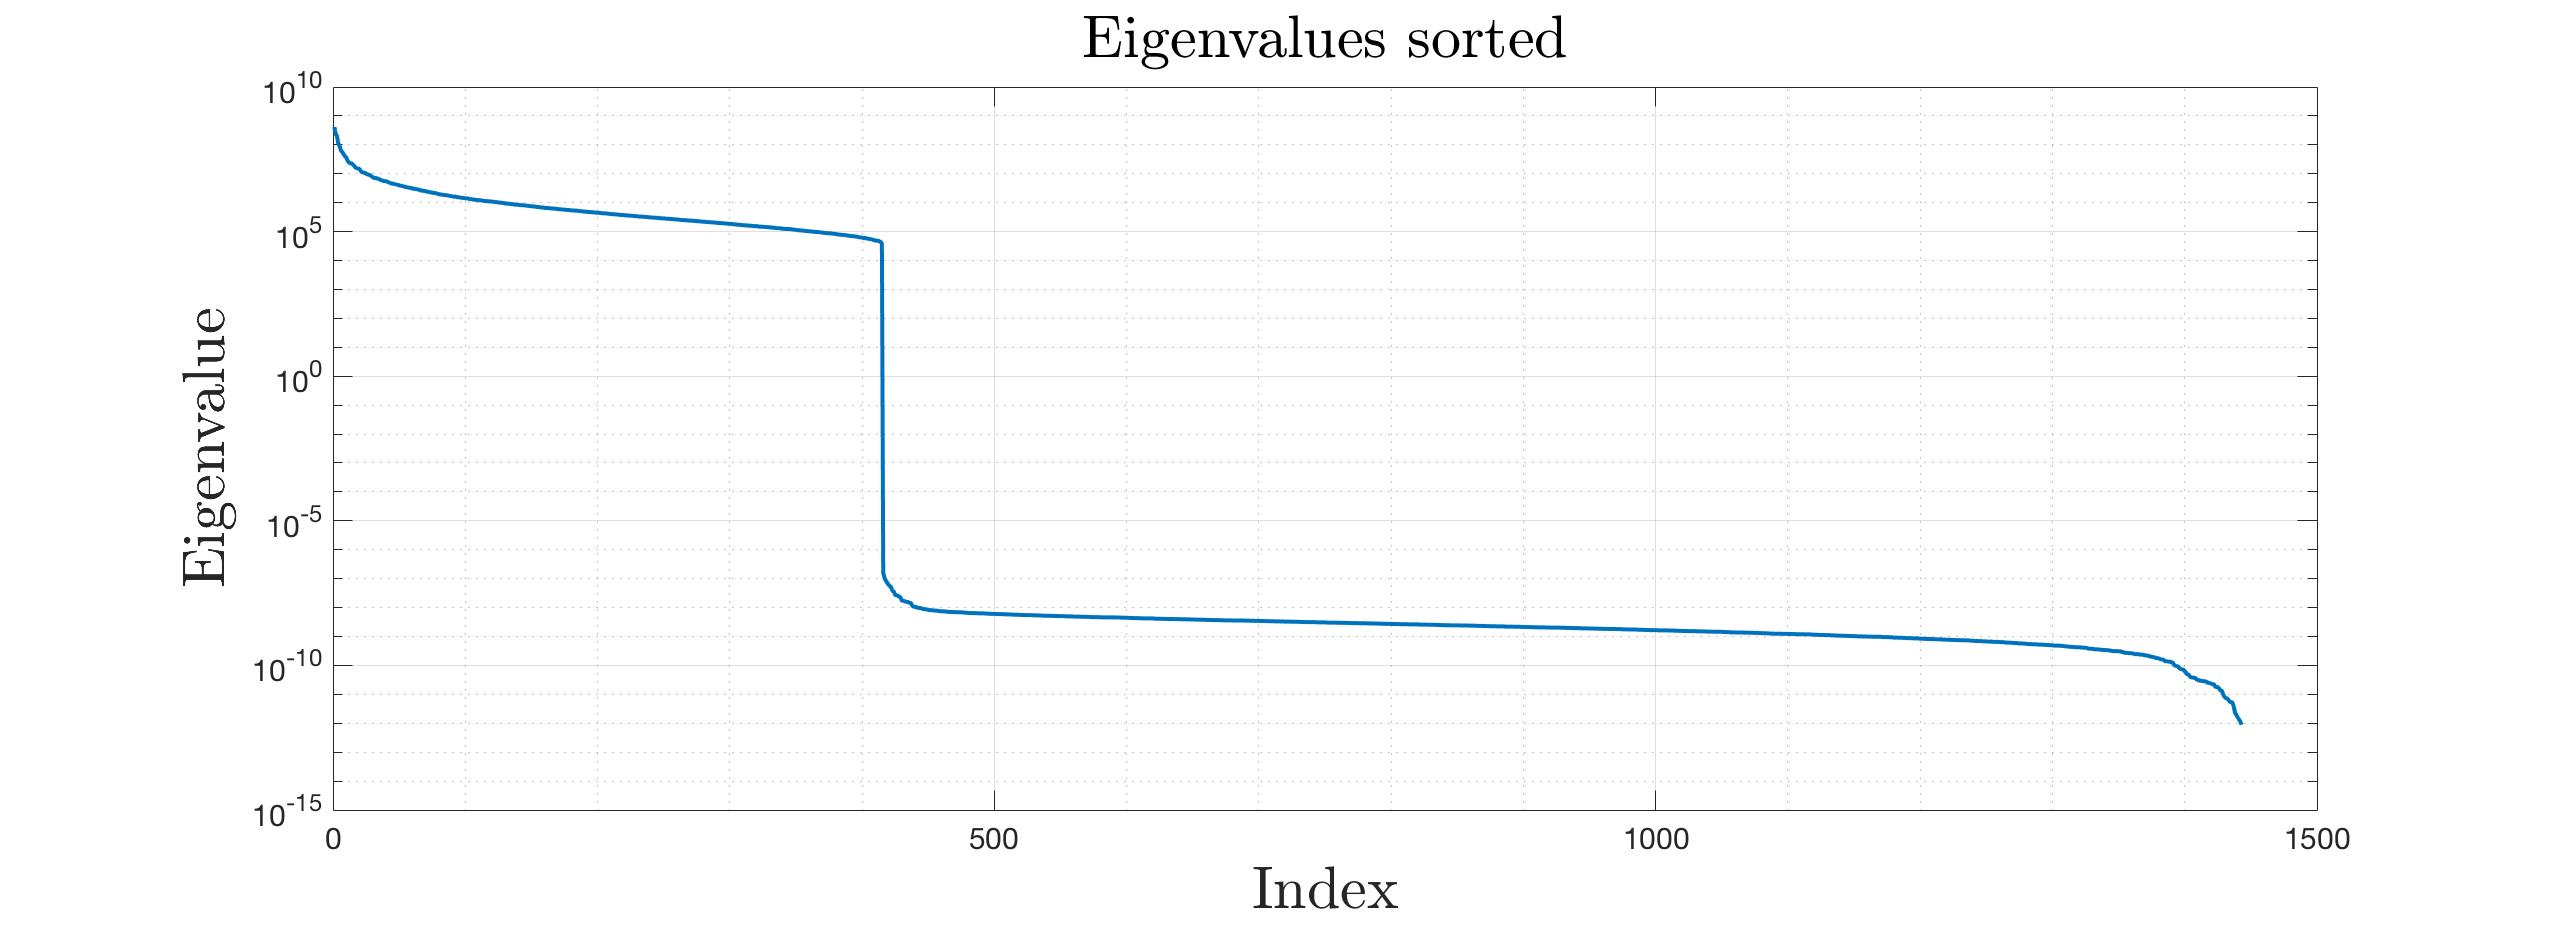
\includegraphics[width=0.5\textwidth]{../results/Q1A_PCA_Eigenvalues}

  \caption{Sorted Eigenvalues of Covariance Matrix $S$ \label{fig:Eig1}}

\end{figure}

It can be seen that first 415 values are much greater than 1. The \nth{416} value is around $10^{-10}$. The three best eigenvectors, or eigenfaces corresponding to the three highest eigenvalues are shown below in Figure \ref{fig:Eig2} . Finally the mean face which was initially subtracted from the face data is shown in Figure \ref{fig:Mean} .


\begin{figure}[H]

\centering
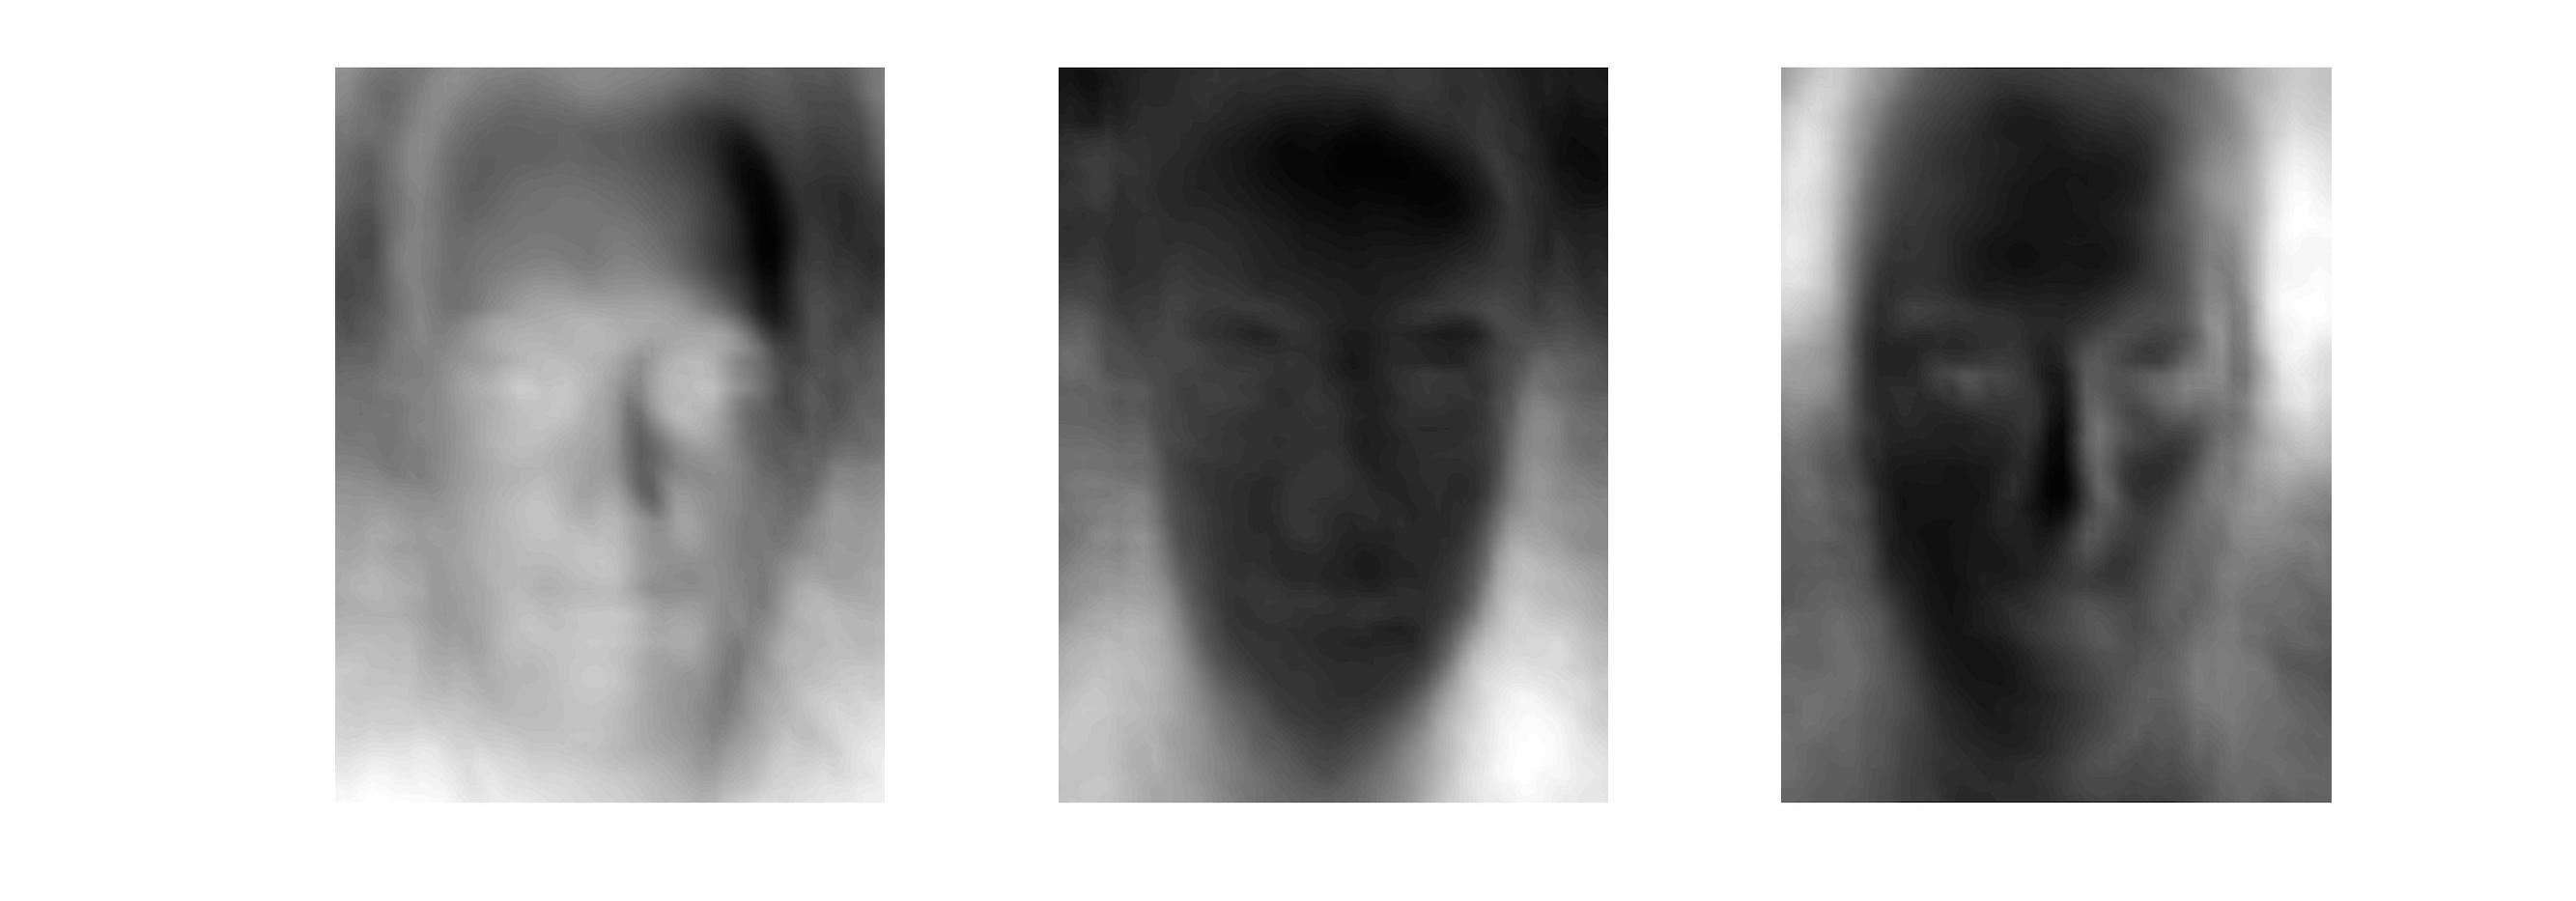
\includegraphics[width=0.5\textwidth]{../results/Q1A_PCA_Eigenfaces}

  \caption{Best 3 Eigenfaces of Covariance Matrix $S$ \label{fig:Eig2}}

\centering
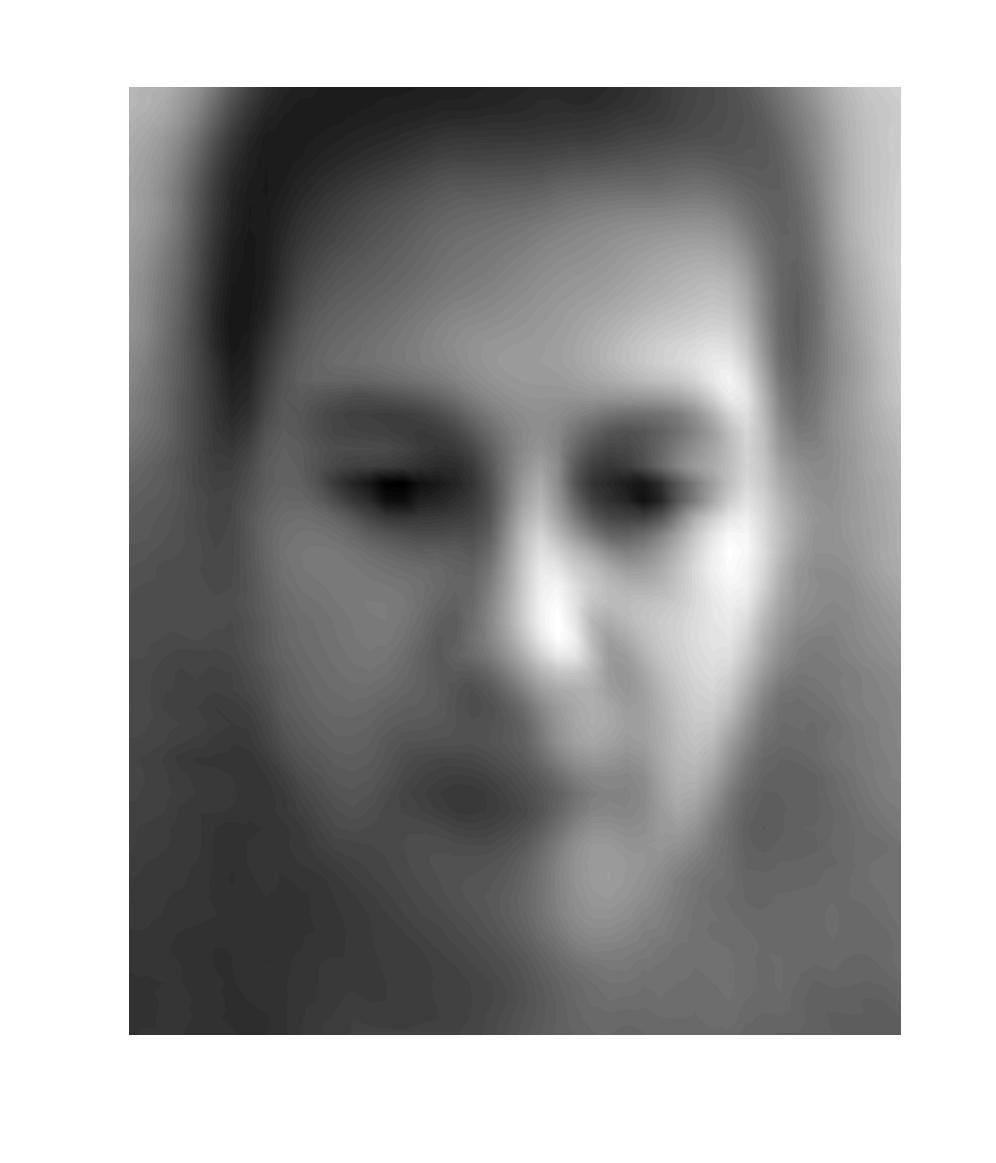
\includegraphics[width=0.15\textwidth]{../results/Q1A_PCA_Mean}

  \caption{Mean Face from {\tt\small training} \label{fig:Mean}}

\end{figure}


The 95\% confidence bound would require us to use 121 eigenfaces. This constitutes a compromise between accuracy and performance, by reducing the problem dimensionality.
\subsubsection{\boldmath$A^TA$} \label{sec:ata}
Alternatively as suggested earlier we could compute a covariance matrix $S_T = \frac{1}{416} \times A^TA$, which now has dimensions of $416 \times 416$ instead of $2576 \times 2576$. We know \cite{Data Mining} that both matrices produce the same (meaningful) eigenvalues. Their plot in the  descending order in Figure \ref{fig:Eig3} proves the above claim.

\begin{figure}[H]
\centering
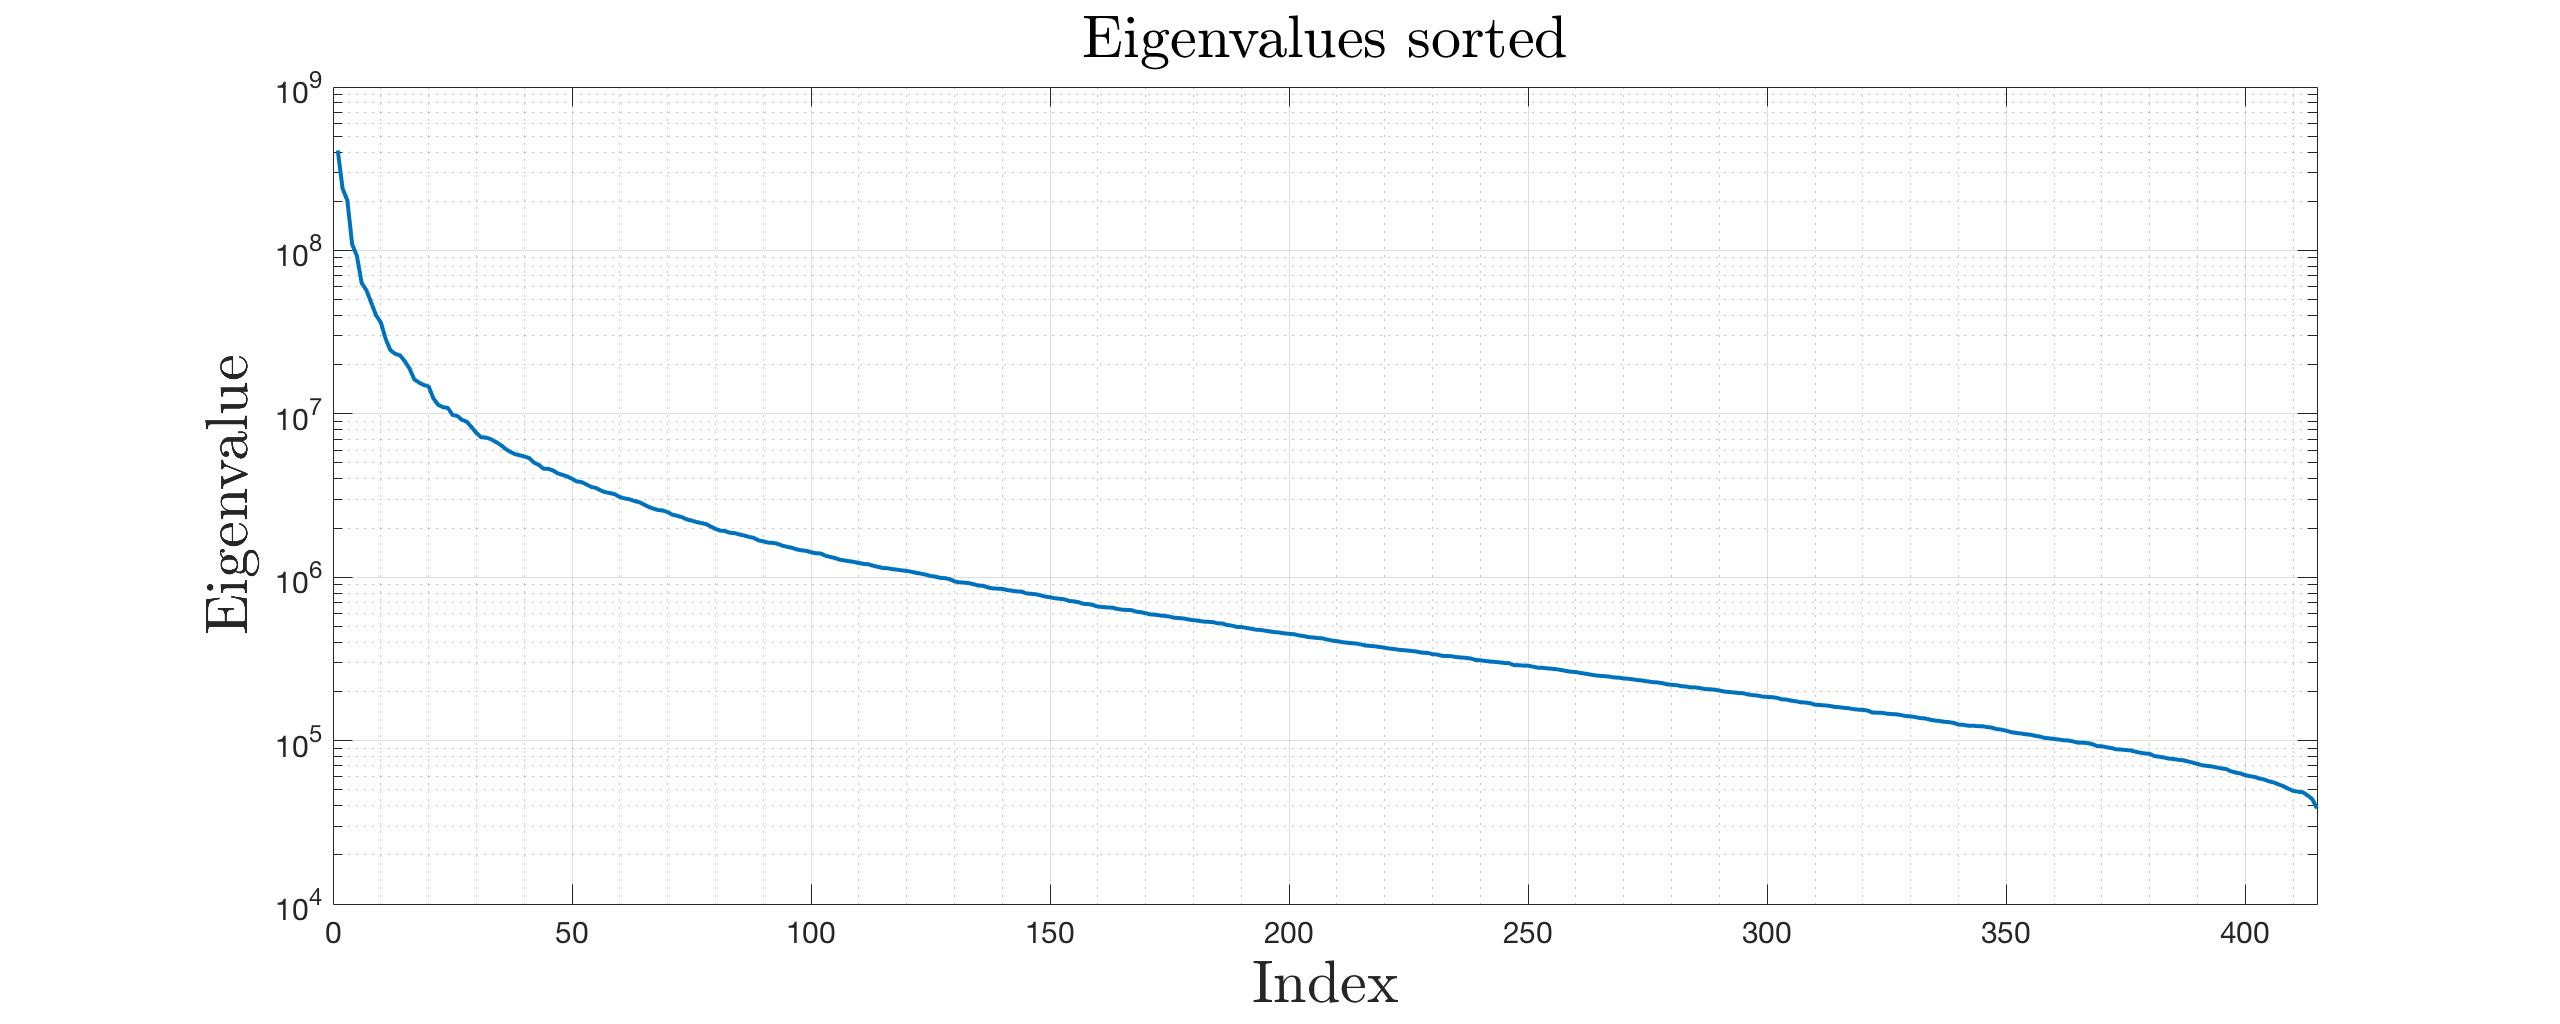
\includegraphics[width=0.5\textwidth]{../results/Q1B_PCA_Eigenvalues}

  \caption{Eignevalues of $S_T$ \label{fig:Eig3}}

\end{figure}
\setlength{\belowdisplayshortskip}{0pt}
\setlength{\abovedisplayshortskip}{0pt}
Figure \ref{fig:Eig3} allows to to deduce that the \nth{416} value is actually zero. If it was non-zero the two methods of calculating a covariance matrix would result in very tiny, yet identical values. However the first method resulted in eigenvalue 416 being equal to $2.3 \times 10^{-10}$, whereas the second method gave a value of $-1.9 \times 10^{-12}$.

We know however that eigenvectors will be different and therefore more computation is required to find the eigenfaces. Starting from:

\begin{equation}
A^TAx = \lambda x
\end{equation}

Let us multiply both sides by $A$:

\begin{equation}
AA^T(Ax) = \lambda (Ax)
\end{equation}

We deduce that the eigenvectors of $AA^T$ are $u_i = Ax_i, \forall \lambda_i \neq 0$, where $x_i$ is the i$^{th}$ eigenvector of $A^TA$. Having thus calculated $x_i$, we must multiply each of the vectors by the original zero-mean matrix {\tt\small training} in order to obtain eigenfaces.

However as we do it, we find that some of the images have inverted colours - i.e. the direction of the vector has been reversed. using Singular Vector Decomposition for any two matrices $AA^T$ and $A^TA$ we can show that:
\begin{equation}
Av_i = \sigma_i u_i
\end{equation}
, where $u_i$ and $v_i$ are the eigenvectors of the two matrices respectively and $\sigma_i$ is the square root of the corresponding eigenvalue. Thus having found $v_i$ we can calculate $u_i = \sfrac{Av_i}{\sigma_i}$. Given that $\sigma_i > 0  \forall i$, $Av_i$ has the effect of reversing the direction of some eigenvectors.
%This is however not an issue, e.g. vectors $x= \begin{bmatrix}
%1&1 \end{bmatrix} $ and $y= \begin{bmatrix}
%-1&-1 \end{bmatrix} $ are parallel. The best 3 eigenfaces are shown in Figure \ref{fig:Eig4} . Note the direction reversal in the middle image.

\begin{figure}[H]
\centering
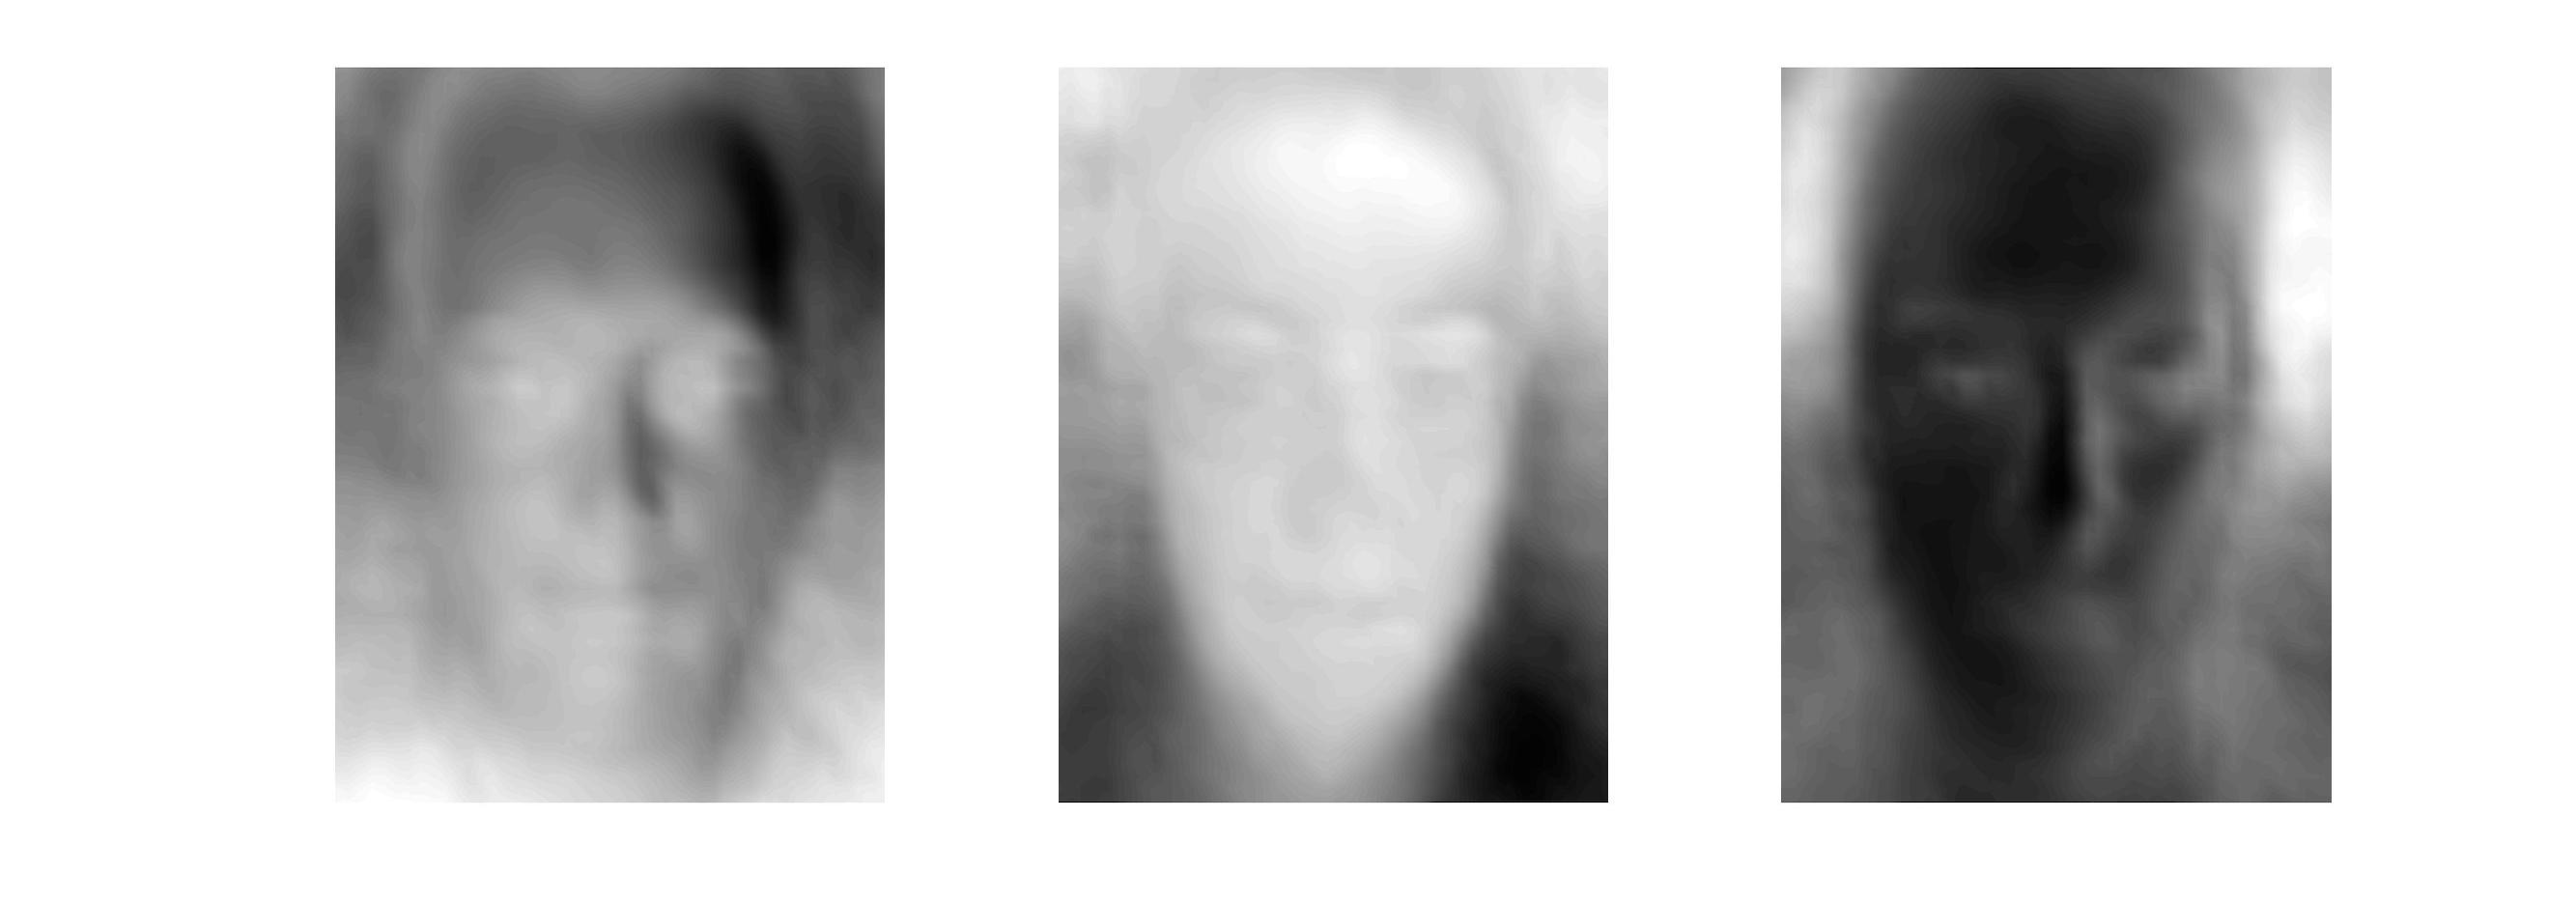
\includegraphics[width=0.5\textwidth]{../results/Q1B_PCA_Eigenfaces}

  \caption{Top 3 Eigenfaces \label{fig:Eig4}}

\end{figure}
\subsubsection{Comparison}

We know that the method presented in section \ref{sec:aat} is accurate. It is however more time consuming to calculate the eigenvectors of matrix with dimensions $2576 \times 2576$ rather than those of a $416 \times 416$ matrix. It is shown \cite{Complex} that eigenproblem complexity is bounded by $O(n^2log(n)+(nlog^2(n))log(b)$, where $b$ is a measure of accuracy in bits $2^{-b}$. However it should be noted that the eigenvectors of the second matrix are not what we are trying to calculate. Thus the latter method introduces an extra step. We have thus timed the full execution of both methods from implementing the {\tt\small eig} function to having a dataset with properly ordered eigenvectors. The results are shown in Table \ref{tab:times1} .

\begin{table}[H]
\begin{center}
\begin{tabular}{||c c||}
\hline
\bf Algorithm & \bf Time\\ [0.5ex]
\hline
 $AA^T$ & 3.59 sec\\ [0.5ex]
\hline
 $A^TA$ & 0.176 sec \\ [0.5ex]
\hline
\end{tabular}
\end{center}
\caption{Computation Time for Both Algorithms} \label{tab:times1}
\end{table}

\section{Applications of Eigenfaces}
\subsection{Face reconstruction}

For the remainder of the work, the second algorithm (\ref{sec:ata}) has been used.

Having determined the PCA bases we are now able to reconstruct faces. We expect that those from the training set will be reconstructed more accurately for any given number of PCA components.

\begin{figure}[H]
\begin{center}
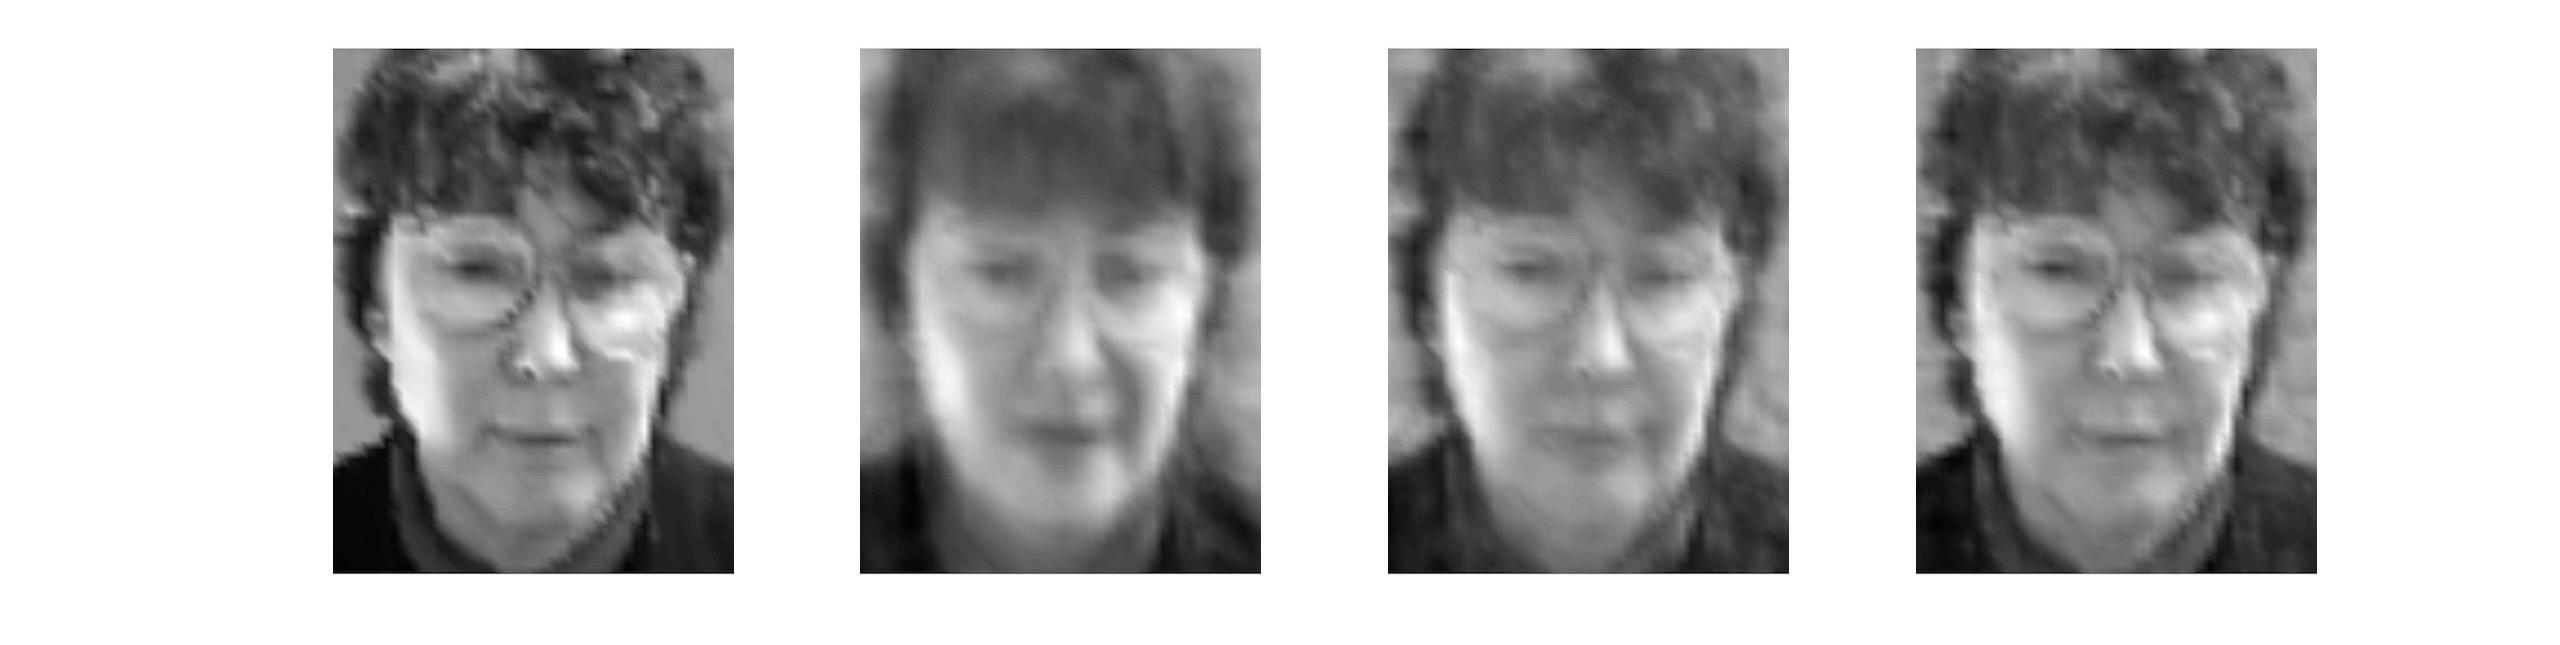
\includegraphics[width=0.5\textwidth]{../results/Train1_reco}

  \caption{Reconstruction of a Training Face: Original, 50 bases, 121 bases, 180 bases \label{fig:RecoTrain1}}
  
  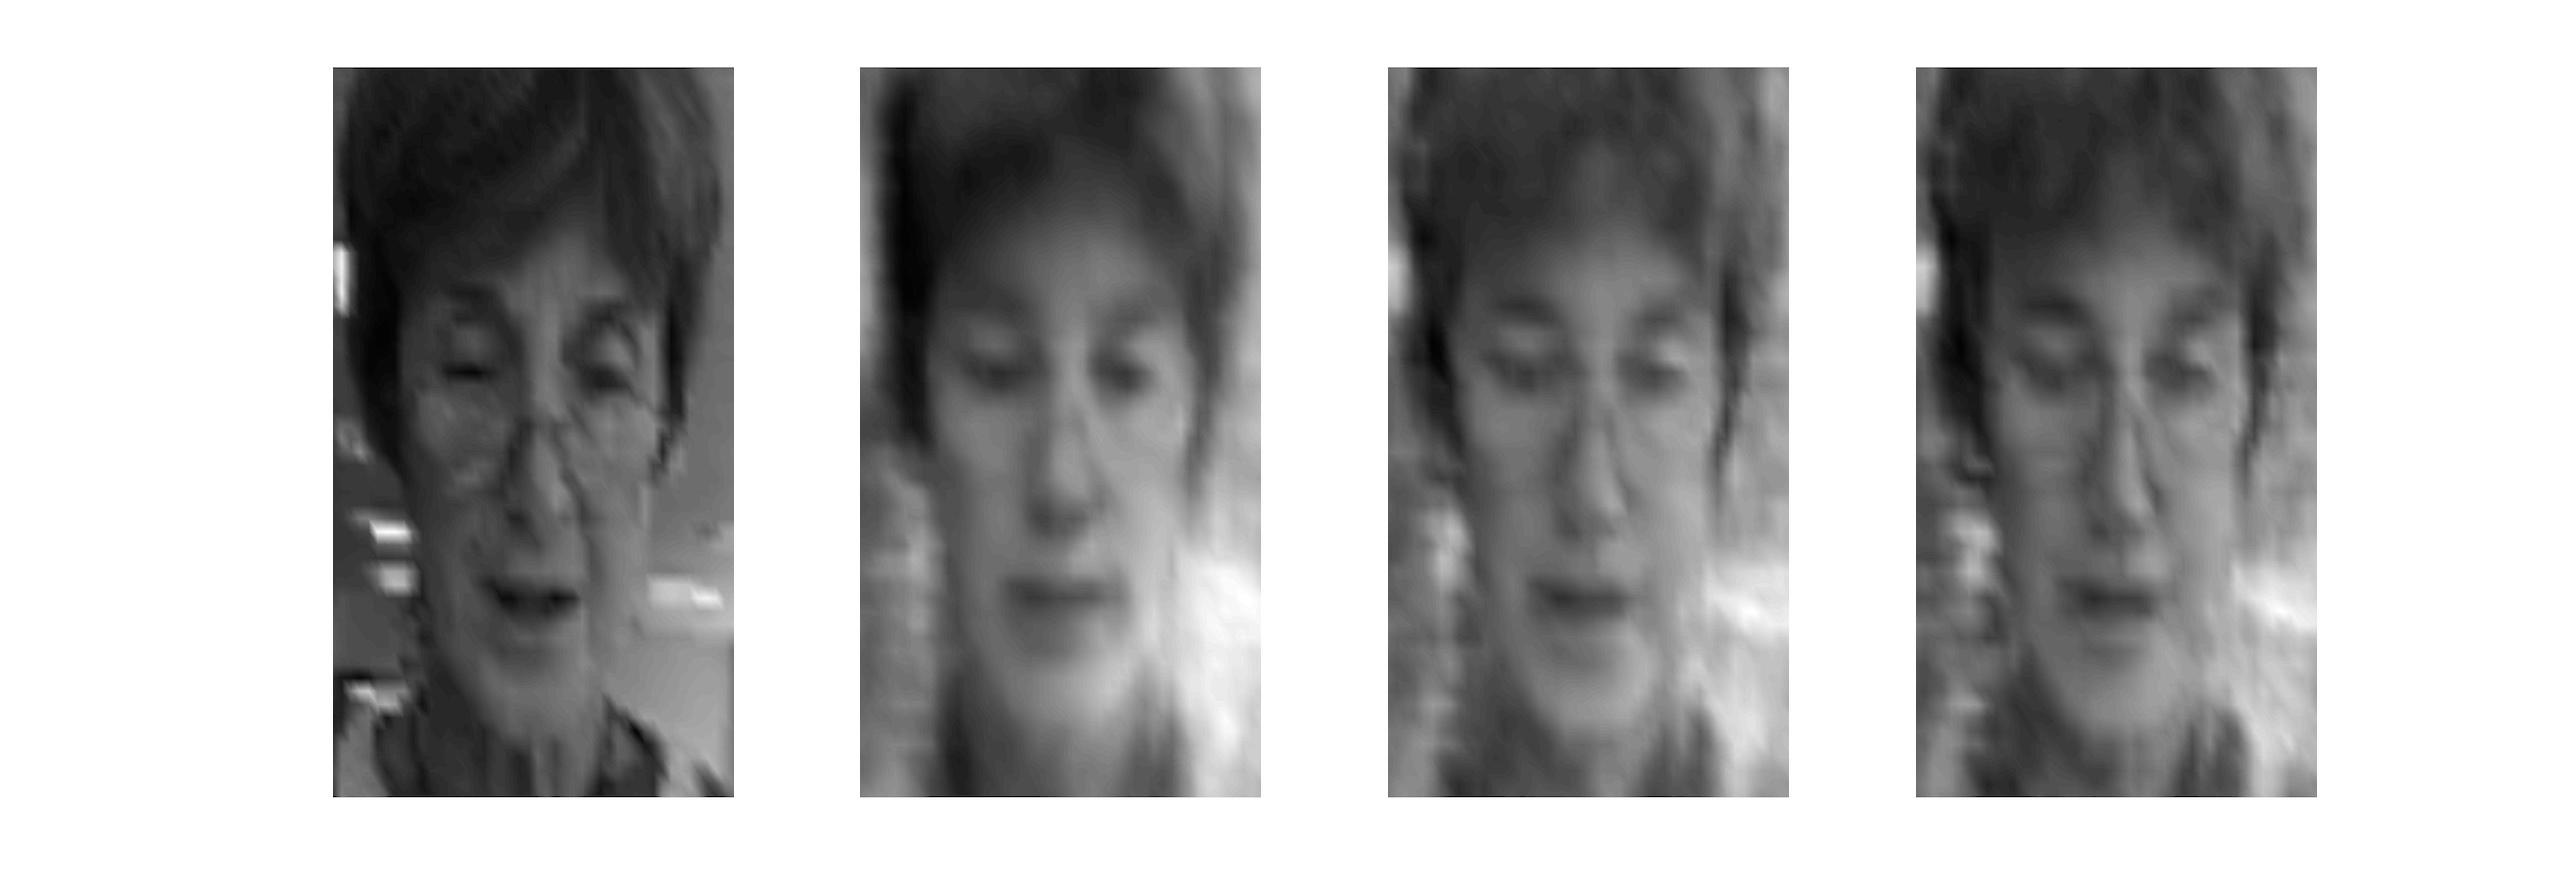
\includegraphics[width=0.5\textwidth]{../results/Test1_reco}

  \caption{Reconstruction of a Test Face: Original, 50 bases, 121 bases, 180 bases \label{fig:RecoTest1}}

    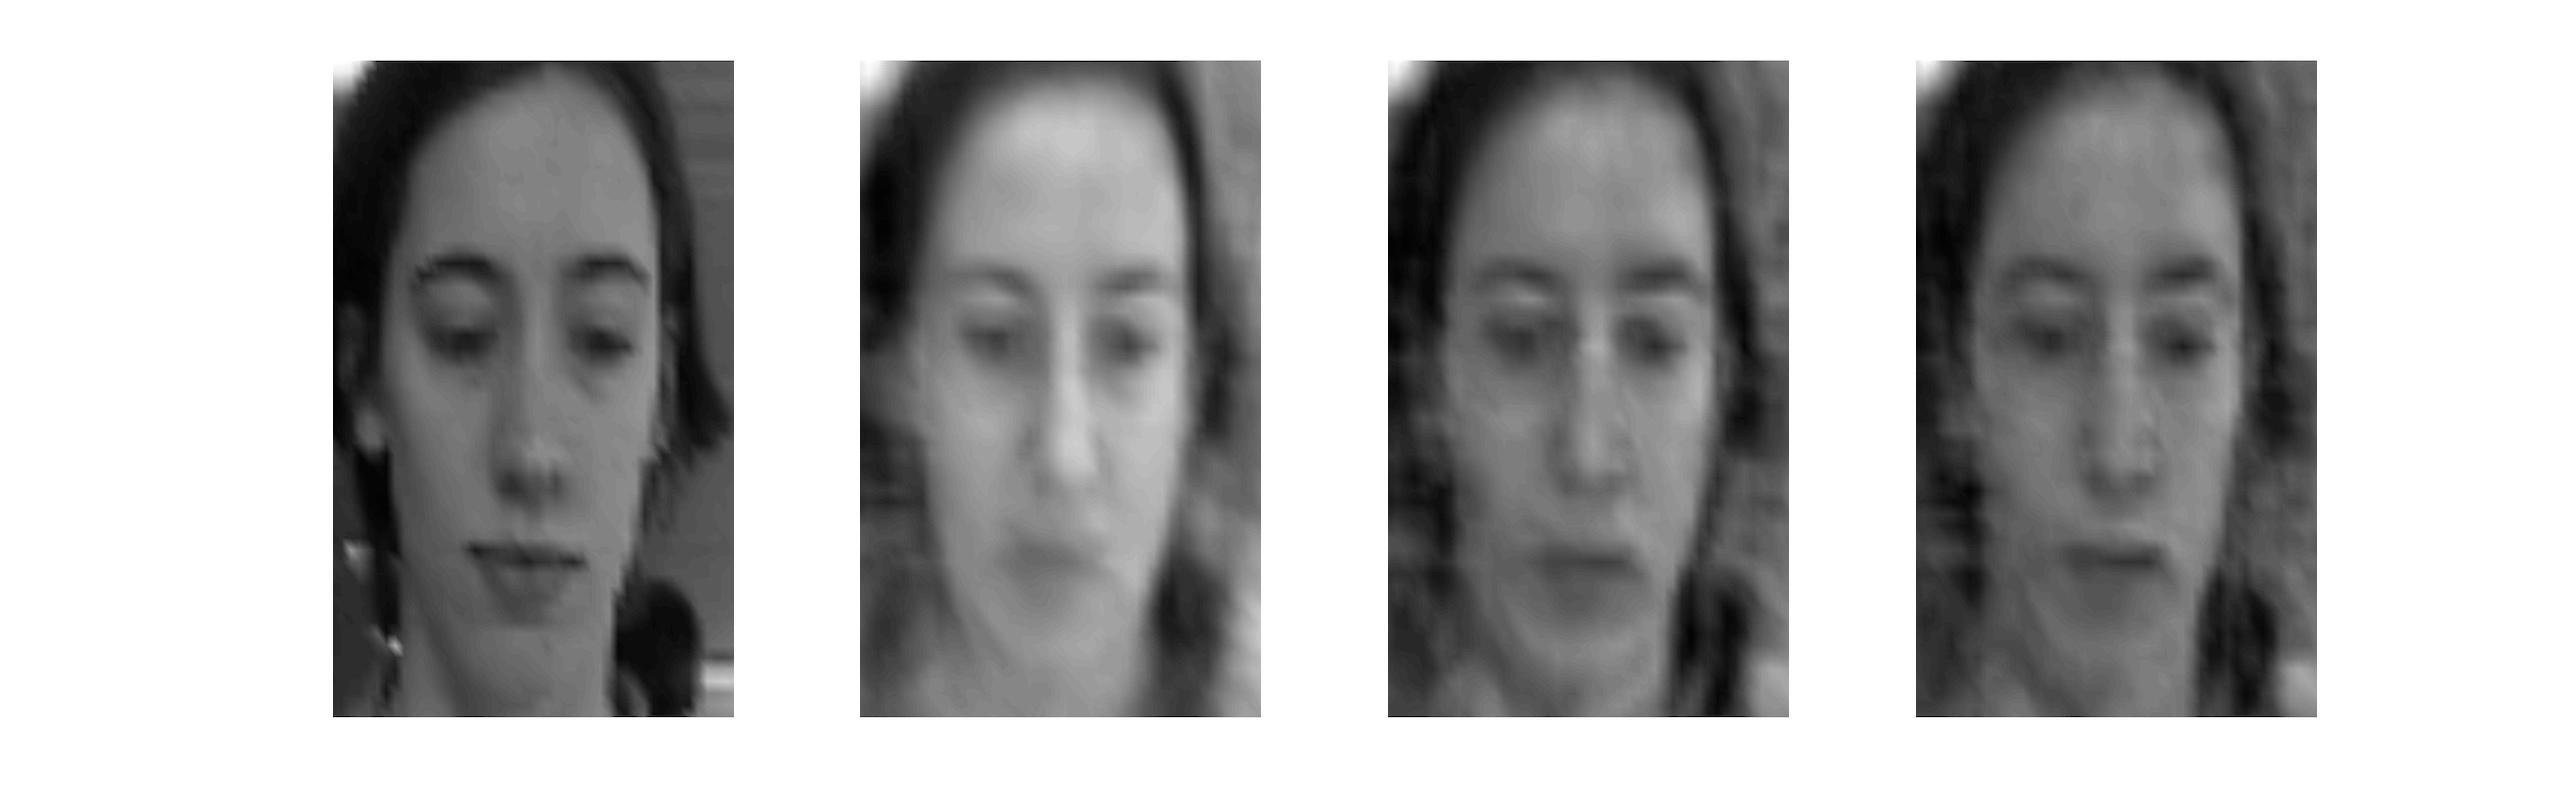
\includegraphics[width=0.5\textwidth]{../results/Test2_reco}

  \caption{Reconstruction of a Test Face 2: Original, 50 bases, 121 bases, 180 bases \label{fig:RecoTest2}}

\end{center}
\end{figure}

The reconstruction errors measured as the Euclidean norm of the difference of two vectors: $Original Face$ and $Reconstructed Face$ of the images shown in Figures \ref{fig:RecoTrain1},  \ref{fig:RecoTest1} and \ref{fig:RecoTest2} are presented in the Table \ref{tab:RecoError} below.

\begin{table}[H]
\begin{center}
\begin{tabular}{||c c c||}
\hline
\bf Image & \bf Number of bases & \bf Reconstruction Error\\ [0.5ex]
\hline \hline
Training Face & 50 & 884.4740 \\ [0.5ex]
\hline
Training Face & 121 & 556.3322\\ [0.5ex]
\hline
Training Face & 180 & 347.7328\\ [0.5ex]
\hline
Training Face & 400 & 18.1174\\ [0.5ex]
\hline \hline
Test Face 1 & 50 & 864.7057\\ [0.5ex]
\hline
Test Face 1 & 121 & 721.7824\\ [0.5ex]
\hline
Test Face 1 & 180 & 676.7093\\ [0.5ex]
\hline
Test Face 1 & 400 & 582.9752\\ [0.5ex]
\hline \hline
Test Face 2 & 50 & 816.2902\\ [0.5ex]
\hline
Test Face 2 & 121 & 649.3541\\ [0.5ex]
\hline
Test Face 2 & 180 & 575.2193\\ [0.5ex]
\hline
Test Face 2 & 400 & 474.1061\\ [0.5ex]
\hline
\end{tabular}
\end{center}
\caption{Reconstruction error for various images and number of PCA bases} \label{tab:RecoError}
\end{table}

Additionally, we can determine the distortion measure of the reconstruction. For any given number of PCA bases, the distortion measure will be the same for any image from the same training set. The distortion measure has been calculated as:
%\begin{equation}
$J = \sum_{n=M+1}^{D} \lambda_n$
%\end{equation}
, where M represents number of PCA bases used to reconstruct the image and D it the total number of eigenfaces. It should also be noted that the eigenvalues are ordered in the descending order s.t. $\lambda_1 > \lambda_2 > ... > \lambda_{M+1} > ... > \lambda_D$.

\begin{figure}[H]
\begin{center}
  
    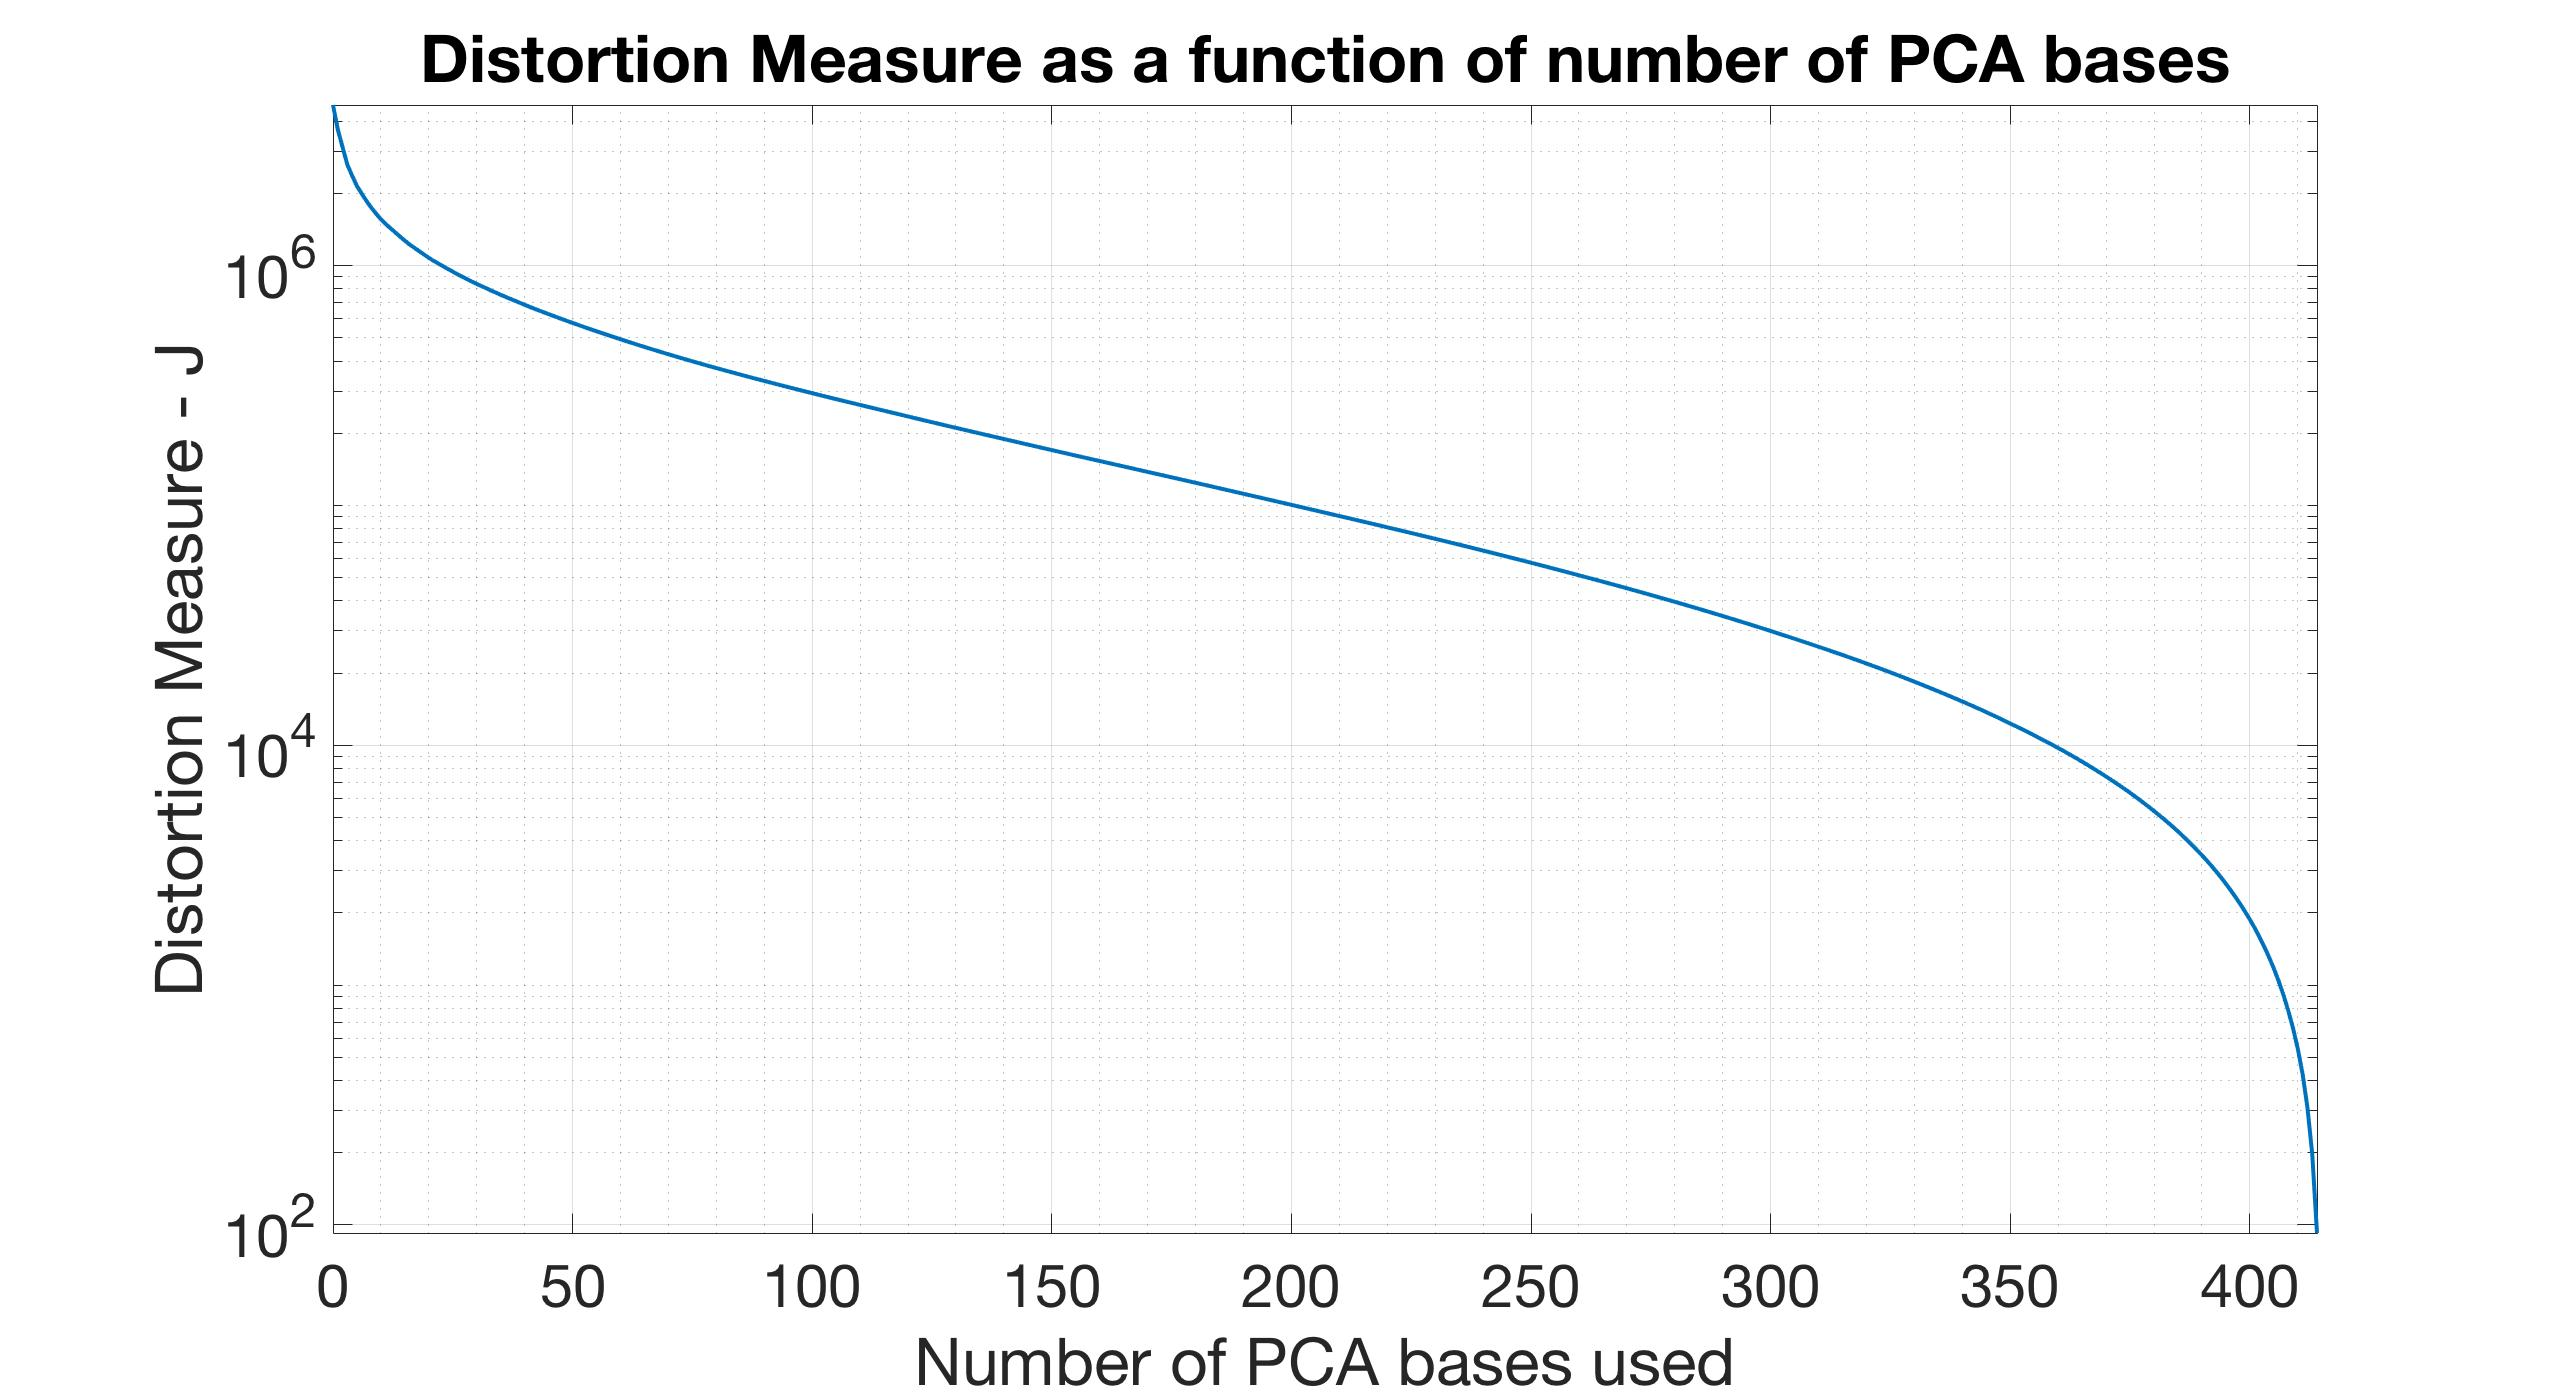
\includegraphics[width=0.5\textwidth]{../results/DistMeasure}

  \caption{Distrtion Measure for varying number of PCA bases \label{fig:DistMeasure}}

\end{center}
\end{figure}
From the Figures \ref{fig:RecoTrain1},  \ref{fig:RecoTest1} and \ref{fig:RecoTest2} we can infer that 121 eigenfaces (the 95\% bound calculated earlier) is sufficient to a human eye in order to assign class to a given image. 50 PCA bases results in a very fuzzy image, though the main characteristics of the class can be identified. Finally, 180 eigenfaces produce a relatively sharp image, though it isn't much different from the one obtained with 121 bases, as shown in Table \ref{tab:RecoError}.

The test results shown in Table \ref{tab:RecoError} show as expected a monotonous trend. As we increase the number of eigenfaces the reconstruction error (or the D-dimensional distance between original and reconstructed images) decreases. We also observe that both face images from the {\tt\small testing} set produce larger errors than the face from {\tt\small training} set for larger amount of PCA bases. The reconstruction error of the training faces can actually reach zero, when we use all of 415 eigenfaces. This however cannot be said about the test faces.

Similarly, we observe that the distortion is monotonously decreasing as we increase number of the PCA bases. This is expected as, with each extra PCA base used to reconstruct we take away the biggest eigenvalue from the total sum.

\subsection{Nearest Neighbour (NN) classification}

In order to perform the PCA-based face recognition, the Nearest Neighbour classification method was used. Having calculated the projections of each normalised training face onto the eigenspace, we could take a new image and classify it into a class. This was done by calculating the new image's projection onto the eigenspace, and compare it to the existing projections. The new image was given the class of the projection that it is closest to. The following classifier equation was used to acheive this:
\begin{equation}
e = min_n ||\omega - \omega_n||,\quad n = 1,...,N
\end{equation}
where $\omega$ is the projection of the new image onto the eigenspace, $\omega_n$ is the projection of the training vector $x_n$ and $N$ is the number of training vectors.

Using this method, each testing vector was classified. With the optimum parameter selection, the classification was successful in $70.1293\%$, and testing images were assigned to the correct class, as shown in Figure \ref{fig:Q2B_NN_success}. However, there were limitations to the classifier. This method works only on how similar the testing image is to one other image, so it is easily fooled by pictures from incorrect classes with similar lighting, or testing images that have a particular difference from the training data, i.e. the removal of the glasses in the failure example in Figure \ref{fig:Q2B_NN_failure}.

\begin{figure}[H]
\begin{center}
  
    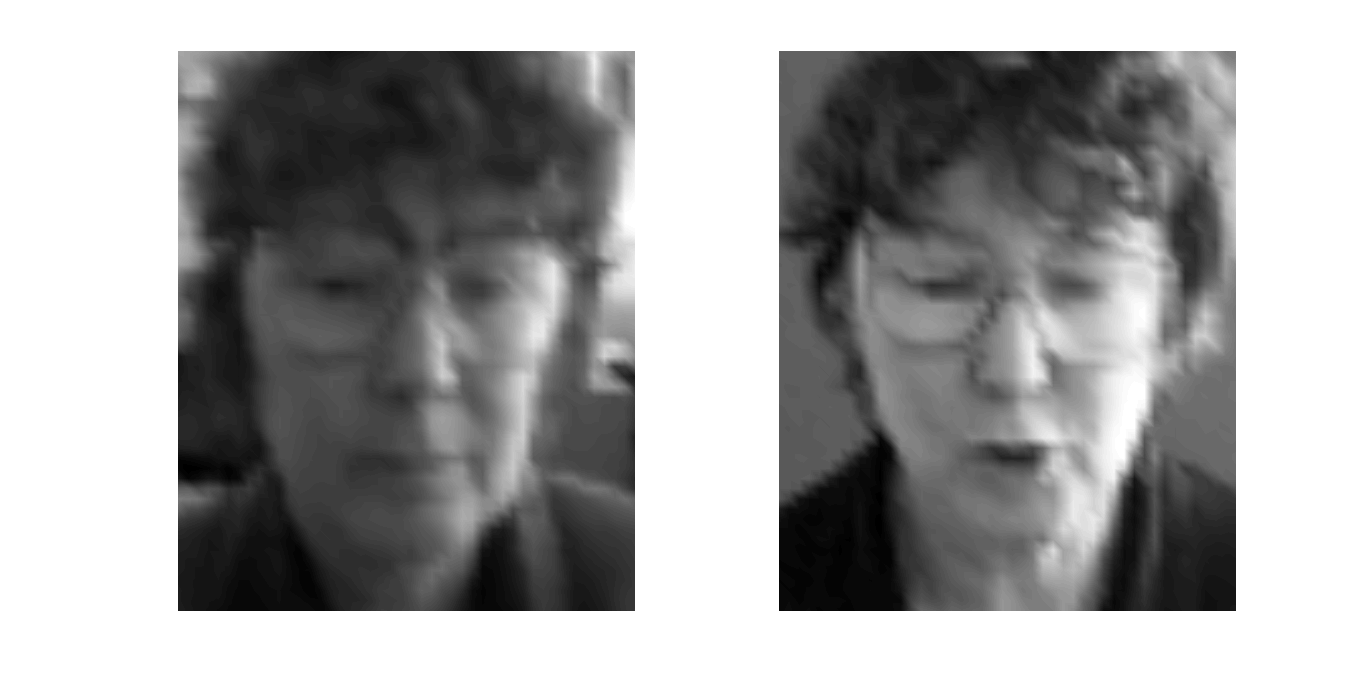
\includegraphics[width=0.3\textwidth]{../results/Q2B_NN_success}

  \caption{Example of a successful classification: Testing Face, Example from Assigned Class \label{fig:Q2B_NN_success}}

\end{center}
\end{figure}

\begin{figure}[H]
\begin{center}
  
    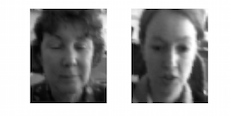
\includegraphics[width=0.3\textwidth]{../results/Q2B_NN_failure}

  \caption{Example of a failed classification: Testing Face, Example from Assigned Class \label{fig:Q2B_NN_failure}}

\end{center}
\end{figure}

Varying the number of eigenvectors used to project vectors onto the eigenspace causes the execution time and success rate of the classifier to change, as can be seen in Table  \ref{fig:Q2B_NN_success}. It can be clearly seen that as the number of eigenvectors increases, the execution time increases, while the success percentage peaks when the number of eigenvectors is 150.

\begin{table}[H]
\begin{center}
\begin{tabular}{||c c c||}
\hline
\bf Num. Eigenvectors & \bf Execution Time /sec & \bf Success \%\\ [0.5ex]
\hline \hline
50 & 0.227370 & 63.4615 \\ [0.5ex]
\hline
100 & 0.232730 & 68.2692 \\ [0.5ex]
\hline
125 & 0.241029 & 69.2308 \\ [0.5ex]
\hline
150 & 0.245756 & 70.1923 \\ [0.5ex]
\hline
175 & 0.263097 & 69.2308 \\ [0.5ex]
\hline
200 & 0.292893 & 69.2308 \\ [0.5ex]
\hline
250 & 0.357959 & 68.2692 \\ [0.5ex]
\hline
\end{tabular}
\end{center}
\caption{Execution time and success percentage for Nearest Neighbour Classifier with different numbers of eigenvalues} \label{tab:NN_table}
\end{table}

\section{Multi-Class SVM}
\subsection{Binary Class SVM}
The Support Vector Machine in the simple form supports binary classification of data. Hence if we train the classifier with 52 classes we will obtain meaningless results. This section is based on the LibSVM Matlab library provided by \cite{LibSVM}. In order to achieve multiclass SVM classification we can implement one of two algorithms: one-versus-one (OVOSVM) or one-versus-all (OVASVM). These two are both based on the binary version of SVM. There are other extensions of SVM which also allow multiclass recognition.
\subsection{One-versus-one SVM}
For $C$ number of classes, one-versus-one SVM technique requires $T = \sfrac{(C-1)}{2}\times C$ trainings and testings as we want to compare each pair of classes and run the test image past the resulting kernels. It can be seen already that this method is computationally expensive. In our case $C=52$ and so $T = 1325$. However each of the kernels is relativley easy to compute as it is made up of 16 training points, due to our data division.

The test image is passed through all 1325 kernels. Each kernel will assign the image to class $j$ or $i$, $1<j<C \quad j<i<C+1$. Those are called votes. For instance if we input an image of class 3, we expect (ideally) that all 51 kernels which are based on class 3 will result  in $3$ being assigned to the image. We then expect that all other kernels will 'randomly' assign other classes, thus making class 3 the highest voted class.
 
\subsection{One-versus-all SVM}
Another method of performing the multiclass SVM classification is to employ the one-versus-all SVM method. Instead of creating 1325 kernels, we only require 52. By taking class $j$ as one part of the kernel, the OVASVM algorithm essentially assumes that the remaining $C-1$ classes are just one class. That way we can examine if the image belongs to class $j$ or the rest. Ideally OVASVM should result in +1 being outputted just once. This assumption could allow us to, on average, halve the computation time, as we wouldn't have to check other kernels if we have found the correct class early on. However this time in order to compute the kernel, we employ all 416 training images, which takes considerably longer.

However, OVASVM's disadvantage is that the classes are no longer balanced. This means that one class contains more data than the other. This affects the way the hyperplane is constructed. Practically, this means that the minority class would be ignored as shown in Figure \ref{fig:SVM_un}. This can be compensated for with changing the way misclassification is penalised - commonly known as class-weighted SVM. Using the LibSVM library we do it by inserting the {\tt\small -wi} flag.
\begin{figure}[H]
\begin{center}
  
    \includegraphics[width=0.4\textwidth]{../results/SVM_unbalanced}

  \caption{Example of unbalanced binary class SVM \cite{SVM_unb}} \label{fig:SVM_un}
\end{center}
\end{figure}

\subsection{Comparison}

{\small
\bibliographystyle{ieee}
\bibliography{egbib}
}

\begin{thebibliography}{9}
\bibitem{Data Mining} 
Inderjit Dhillon. 
\textit{CS 391D Data Mining: A Mathematical Perspective Fall 2009}. 
The University of Texas at Austin, September 2009.

\bibitem{Complex} 
Victor Y.Pan, Zhao Q. Chen, Ailong Zheng. 
\textit{The Complexity of the Algebraic Eigenproblem}. 
Lehman College and Graduate Center, CUNY, NY, December 1998

\bibitem{LibSVM}
Chang, Chih-Chung and Lin, Chih-Jen
\textit{LIBSVM: A library for support vector machines}
ACM Transactions on Intelligent Systems and Technology, vol. 2, iss. 3, 2011, 27:1--27:27
Software available at \url{http://www.csie.ntu.edu.tw/~cjlin/libsvm}

\bibitem{SVM_unb}
D. Cournapeau
\textit{3.2. Support Vector Machines}
scikits.learn developers (BSD License), 2010

\end{thebibliography}
\end{document}
